\section{Motivation}
\label{sec: motivation}
High Performance Computing (HPC) applications process large amounts of data that have to be written (read) to (from) large shared files residing in the global parallel file system. In order to make large datasets manageable, these are usually partitioned into smaller sub-sets and assigned to available cores for parallel processing. Complex datasets such as N-dimensional arrays are logically flattened into a linear sequence of bytes and striped across several I/O targets for best performance. This results in the loss of the original spatial locality, as shown in Figure~\ref{fig: small-io}. 
\begin{figure}[!htb]
\centering
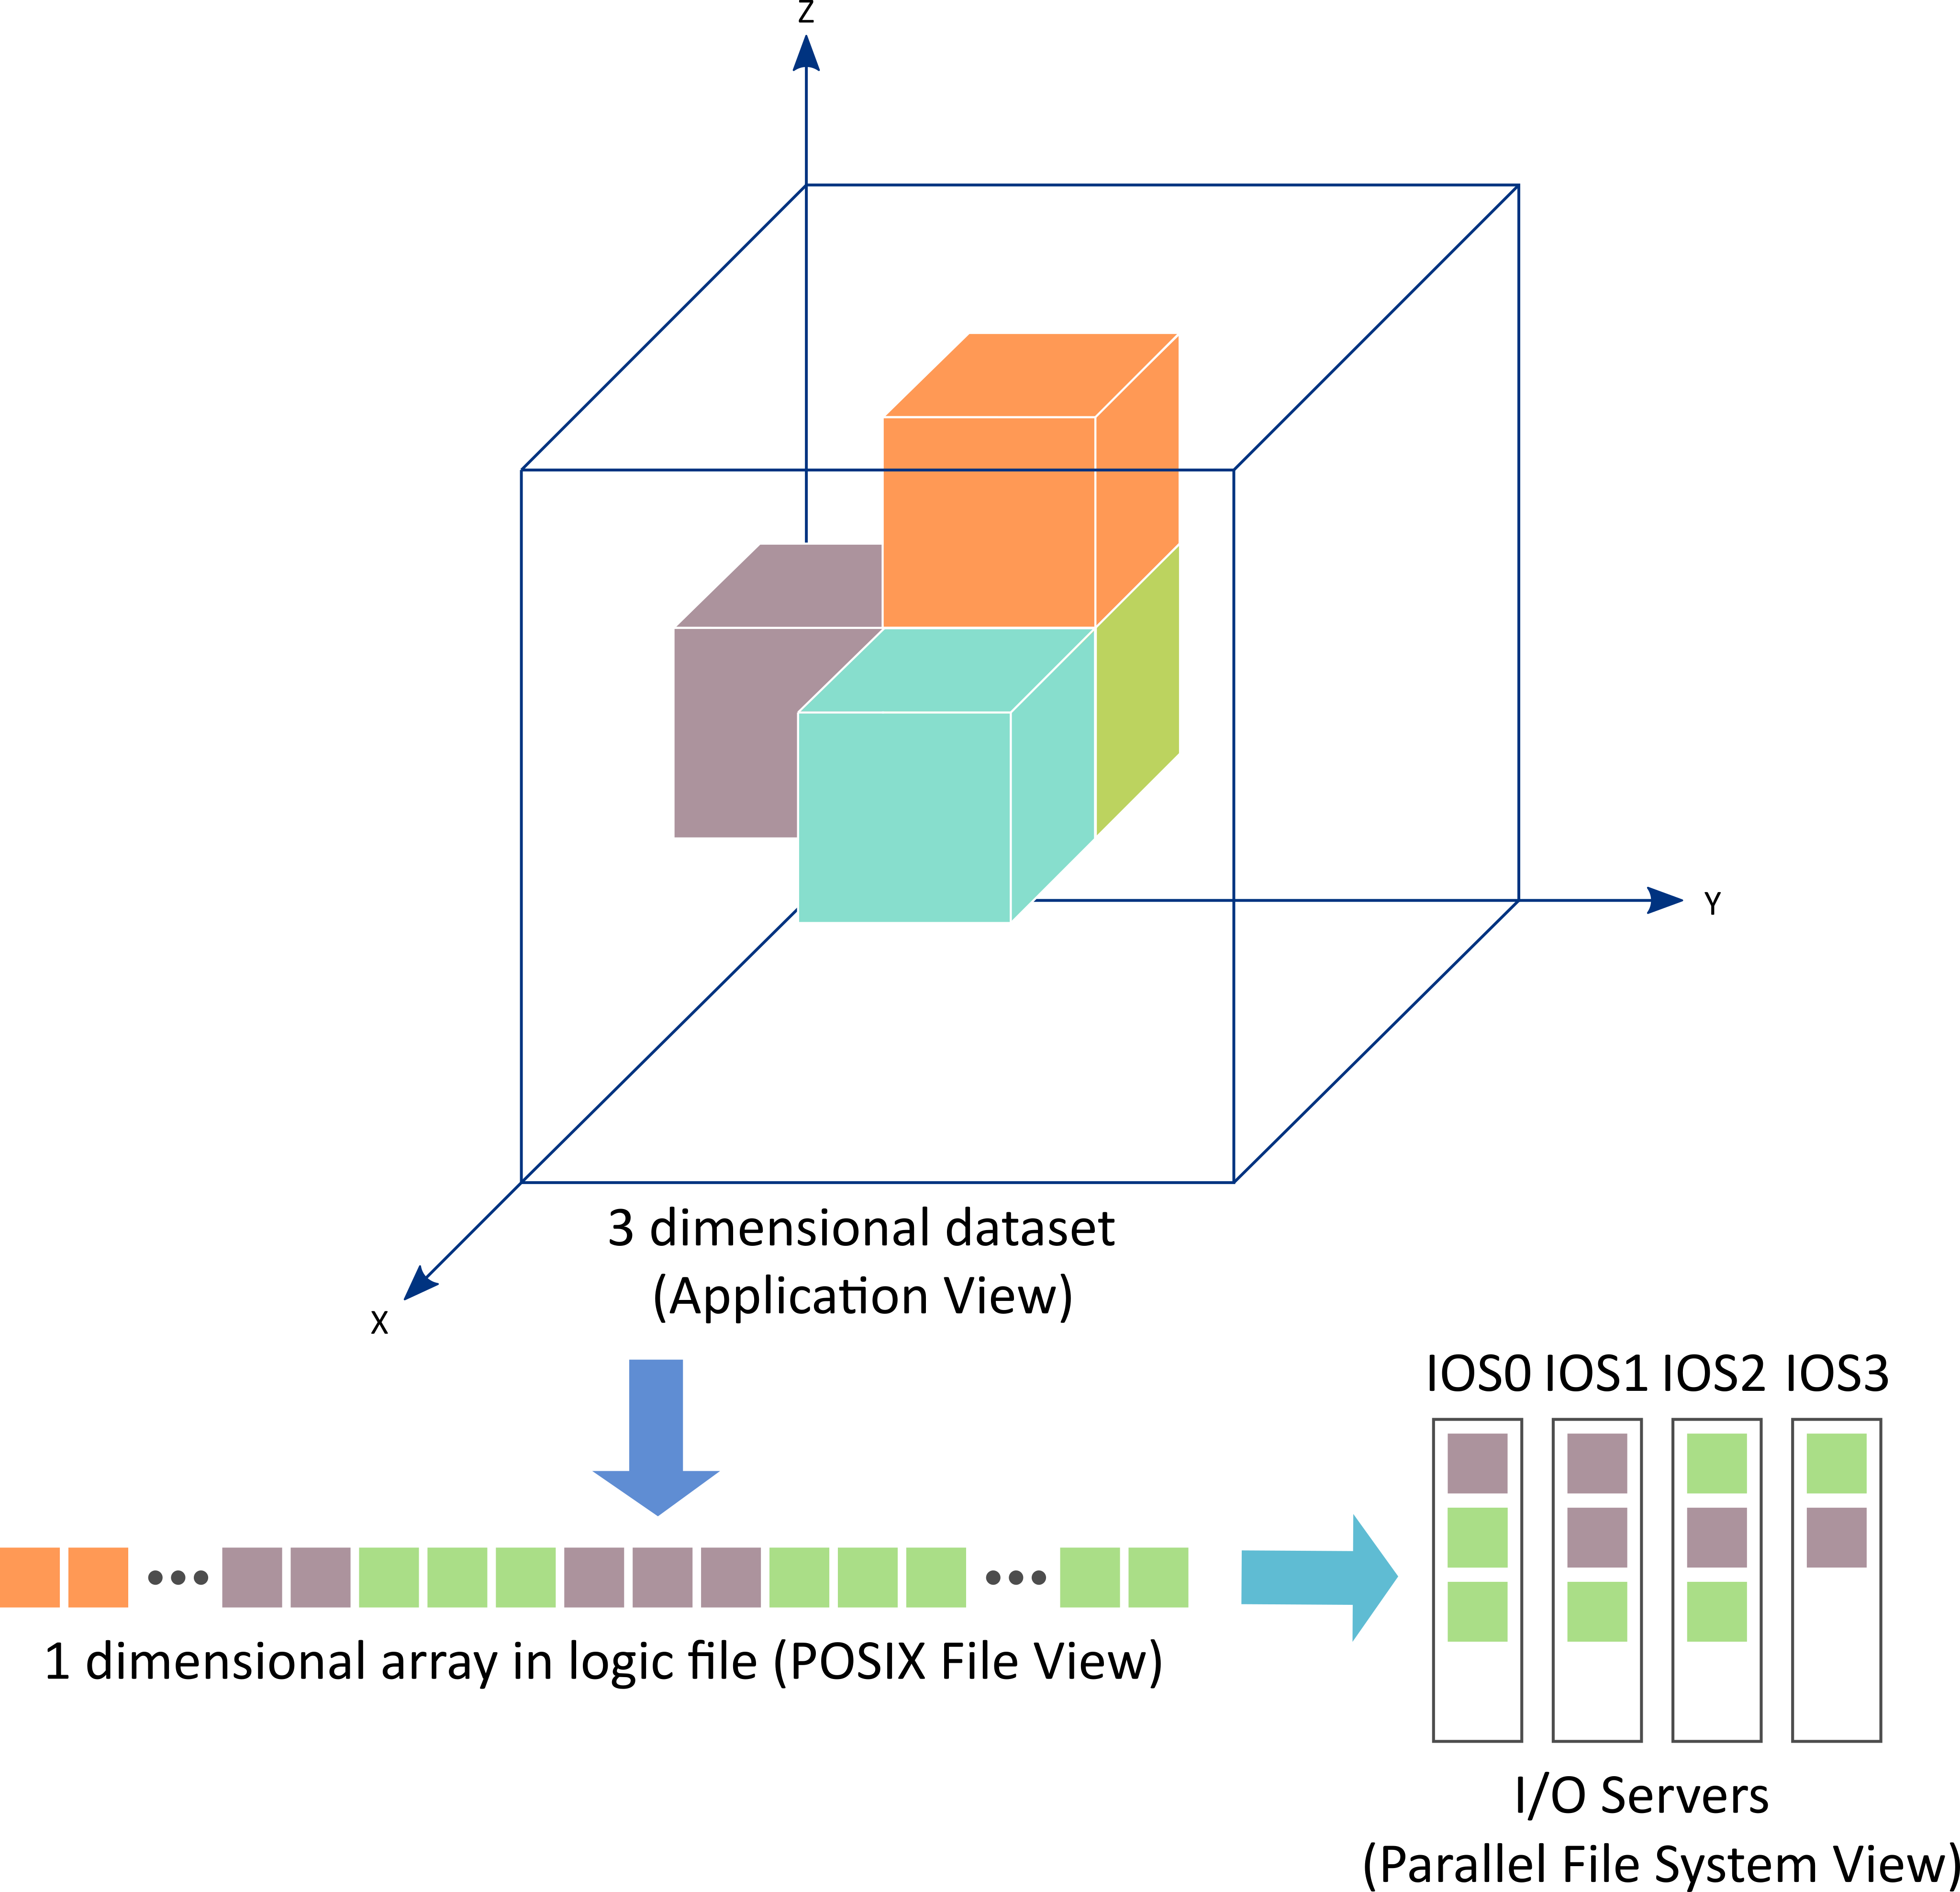
\includegraphics[width=\textwidth]{chapters/chapter3/figures/small-io}
\caption{Example of how a 3-Dimensional dataset is represented logically in the file as a sequence of bytes and how it is finally translated in the parallel file system.}
\label{fig: small-io}
\end{figure}
Due to this characteristic, accesses to spatially contiguous regions translate into non-contiguous accesses to the file. Therefore, applications generating a large number of small, non-contiguous I/O requests to the parallel file system usually experience degradation of I/O performance. Such performance degradation is known as the `small I/O problem' and is related to the fact that parallel file systems provide best I/O bandwidth performance for large contiguous requests, while they typically provide only a fraction of the maximum available bandwidth in the opposite case~\cite{ChingCLP06}~\cite{HeSSYT11}. This is due to the large number of Remote Procedure Calls (RPCs) generated by the file system clients overwhelming I/O servers, the resulting high number of hard disk head movements in every I/O target (seek overhead) and, ultimately, to the restrictions imposed by the POSIX I/O write semantic that generates lock contention in the file systems' blocks.

Having recognised the small I/O problem, collective I/O was proposed by the MPI-IO community~\cite{ThakurGL99}. Collective I/O exploits global I/O knowledge in parallel I/O to a shared file. This knowledge is used to build an aggregated view of the accessed region in the file and coalesce all the corresponding small non-contiguous requests into a smaller number of large contiguous accesses, later issued to the parallel file system. File system accesses are orchestrated in such a way that only a subset of the available processes actually performs I/O. These processes are called `aggregators', because they gather and aggregate all the requests on behalf of the other processes, whose only role in this case is to send (receive) data to (from) aggregators.

In conclusion, collective I/O can convert many small random accesses into large sequential accesses to the I/O subsystem, reducing the actual number of I/O requests that need to be accounted for by the I/O stack. Even when processes generate large I/O requests, it might be still beneficial to coordinate them to reduce parallel file system block locking contention as well as concurrency level on data servers. This mechanism effectively adapts the I/O pattern to the characteristics of the file system, extracting maximum performance from it.
Figure~\ref{figure: coll_io} exemplifies the basic collective I/O mechanism just described. In the figure there are six processes, four of which play the role of aggregators. Collective I/O proceeds in two phases: `data shuffling' and `data I/O'. Data shuffling takes place between all the processes and aggregators and is aimed to build the logically contiguous file regions (or file domains) that will be later accessed during the data I/O phase.

Two phase I/O has a number of problems that limit its scalability. The main issues are: (\textbf{a}) global synchronisation overhead between processes exchanging data, where I/O is bottlenecked by the slowest aggregator process~\cite{WeikuanV08}, (\textbf{b}) aggregators' contention on file system stripes (primarily due to stripe boundary misalignment of the file domains and the underlying file system locking mechanism\footnote{In current ROMIO versions the ADIO driver for Lustre can detect and align file domains to stripe boundaries thus avoiding stripe collisions. A new ADIO driver for BeeGFS supporting the same functionality has been developed in the course of this work.})~\cite{LiaoA08}, (\textbf{c}) aggregators' contention on I/O servers (related to inefficient file domain partitioning strategy), (\textbf{d}) pressure that large collective buffers can have on the memory system (due to scarce amount of available memory per single core in current and future large scale HPC clusters), and (\textbf{e}) high memory bandwidth requirements due to the large number of data exchanges between processes and aggregators~\cite{YinYTY12}. There is also a mismatch between logical file layouts and the collective I/O mechanism, which does not seem to take the physical data layouts into consideration~\cite{YongXTRG11}~\cite{XuechenJD09}.
\begin{figure}[!htb]
  \centering
  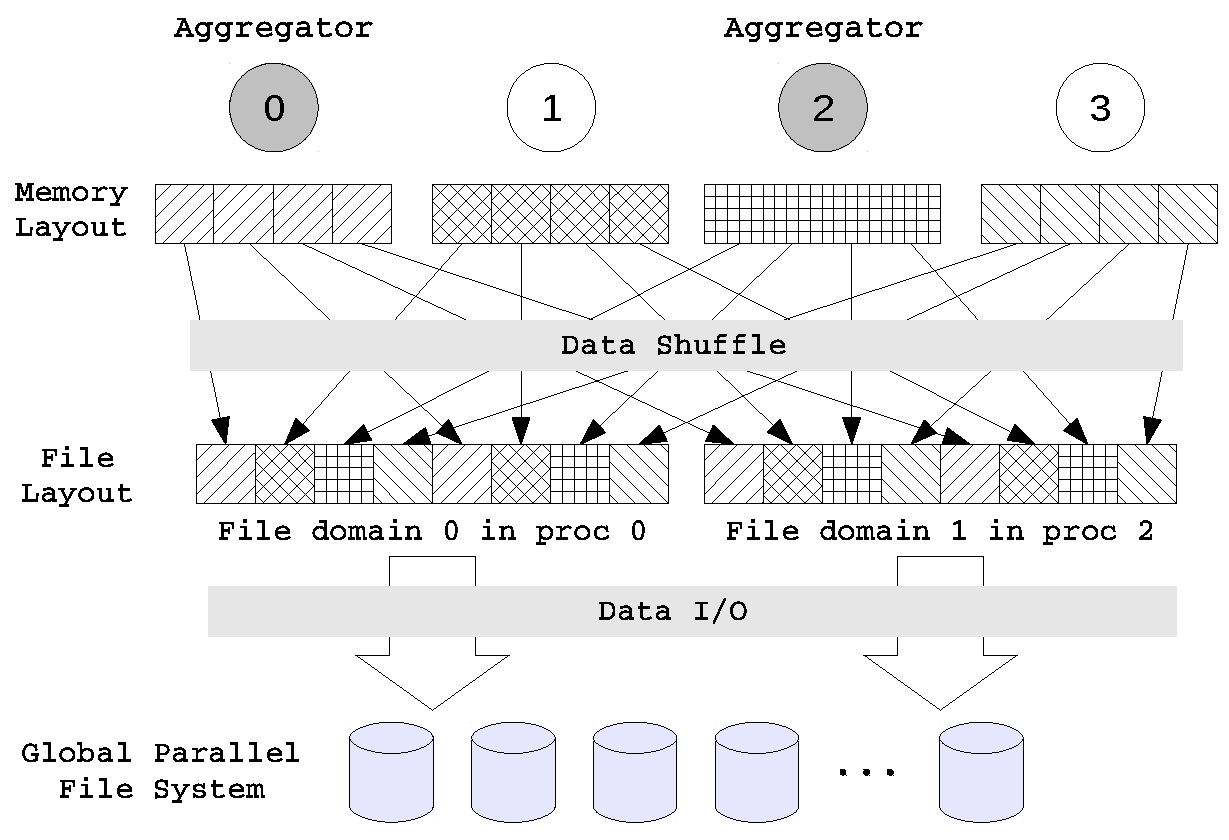
\includegraphics[width=0.6\textwidth]{chapters/chapter3/figures/coll-io}
  \caption{Collective I/O write example. A data set is partitioned and assigned to six processes. Four of them work as aggregators writing data to the global file system.}
  \label{figure: coll_io}
\end{figure}

Nowadays solid state drives (SSDs) are becoming more affordable and many HPC systems provide SSDs attached to compute nodes. Despite the fact that these devices formally provide an additional tier in the storage hierarchy, they are mostly used to store local data and rarely exploited for parallel I/O. As part of the Exascale10 (E10)~\cite{e10} initiative in the DEEP-ER~\cite{deep-er} project, we explore the benefits that the usage of such fast devices can bring when writing collectively to a shared file.

We integrate local storage resources attached to compute nodes (non-volatile memory devices) as persistent cache layer in ROMIO, providing all the additional infrastructure required to asynchronously flush the content of the cached data to the global file system, while keeping the MPI-IO consistency semantics. The new persistent cache layer is fully integrated inside ROMIO and can be easily accessed through a set of newly defined MPI-IO hints.

We show how when using local SSDs, if the number of aggregators is selected properly, significantly better I/O performance can be achieved compared to the case in which only the global file system is used. Contrarily, if the number of aggregators is not properly selected, I/O performance can even degrade. The additional cache layer also delivers more stable response times, reducing the impact of global synchronization on collective I/O, thus addressing point (\textbf{a}) previously discussed, and can reduce the memory pressure in systems with scarce amounts of main memory per core, thus addressing point (\textbf{d}).

The remainder of this chapter is organised as follows. In Section~\ref{sec: concept} we present the concept and design of the ROMIO caching layer and the new hints extensions supporting it, along with all the corresponding semantics implications, in Section~\ref{sec: evaluation} we show the benefits of collective I/O using different benchmarks, in Section~\ref{sec: related} we present collective I/O related works and finally in Section~\ref{sec: conclusion} we draw conclusions and discuss future developments.
